\documentclass[11pt,a4paper]{article}

\usepackage{geometry}
 \geometry{
 a4paper,
 total={150mm,237mm},
 left=30mm,
 top=30mm,
 }

% cf. http://tex.stackexchange.com/questions/50182/subtitle-with-the-maketitle-page
\usepackage{titling}
\newcommand{\subtitle}[1]{%
  \posttitle{%
    \par\end{center}
    \begin{center}\large\textbf{#1}\end{center}
    \vskip0.5em}%
}

\usepackage{color}
\usepackage{graphicx}
\usepackage{subcaption}

\usepackage[utf8]{inputenc}
\usepackage[lf]{venturis} %% lf option gives lining figures as default; 
\usepackage[T1]{fontenc}
\usepackage{beramono}
\usepackage{csquotes}
\usepackage[UKenglish,german]{babel}

\usepackage{fancyvrb}

\widowpenalty10000  % http://tex.stackexchange.com/questions/4152/how-do-i-prevent-widow-orphan-lines
\clubpenalty10000

\title{The SysSon Platform}
\subtitle{Technical Report TR-2016-11-1\\Institute of Electronic Music and Acoustics, Graz\\(Status: completed)}
\author{Hanns Holger Rutz}
% \date{09-Feb-2016}
\date{November 2016}

% cf. https://tex.stackexchange.com/questions/94126/change-font-to-only-section-and-subsection-of-my-document
%\usepackage{titlesec}
%\titleformat{\chapter}[display]
%  {\fontfamily{pag}\selectfont\huge\bfseries}
%  {\chaptertitlename\ \thechapter}
%  {20pt}
%  {\Huge}
%\titleformat{\section}
%  {\fontfamily{pag}\selectfont\bfseries\Large}
%  {\thesection}
%  {1em}
%  {}
%\titleformat{\subsection}
%  {\fontfamily{pag}\selectfont\bfseries\Large}
%  {\thesection}
%  {1em}
%  {}

\usepackage[backend=biber,authordate]{biblatex-chicago} % citereset=chapter
%\usepackage[backend=biber,natbib,isbn=false,useprefix=true,sorting=ydnt]{biblatex-chicago} % citereset=chapter
\addbibresource{all.bib} % add a bib-reference file
\addbibresource{rutz.bib} % add a bib-reference file

% warning: https://tex.stackexchange.com/questions/313477/
% \usepackage{csquotes}

\usepackage{tabularx}
% cf. https://tex.stackexchange.com/questions/84400/table-layout-with-tabularx-column-widths-502525
\newcolumntype{s}{>{\hsize=1cm}X}

% says you should load after babel and fontspec
\usepackage[shrink=10, babel=true]{microtype}	% http://tex.stackexchange.com/questions/141852/latex-allows-line-break-between-concluding-em-dash-and-comma-before-a-new-sub-cl/141854#141854

% has to come first for full scale TeX voodoo bullcrap
\usepackage{hyperref}
% get rid of the horrible coloured boxes around links
\hypersetup{
    colorlinks,%
    citecolor=black,%
    filecolor=black,%
    linkcolor=black,%
    urlcolor=black
}
% has to come after frickin hyperref
\VerbatimFootnotes

\newcommand{\todo}[1]{\colorbox{yellow}{\textsc{todo}: #1}}

\newcommand{\quot}[1]{\guillemotleft {#1}\guillemotright}

\newcommand{\worktitle}[1]{\textit{#1}}

\newcommand{\workentry}[2]{\vspace{7.5pt}\noindent\textbf{#1} (#2)}
\newcommand{\workentrySel}[2]{\vspace{7.5pt}\noindent\textbf{#1}$*$ (#2)}

\newcommand{\figref}[1]{Fig.~\ref{#1}}

\newcommand{\software}[1]{\textit{#1}}

\newcommand{\sysson}[0]{SysSon}
\newcommand{\syssonVersion}[0]{1.8.0}
\newcommand{\syssonVersionS}[0]{1.8.0-SNAPSHOT}

\newcommand{\artefacts}[0]{\textsc{Artefacts:}}
\newcommand{\assessment}[0]{\textsc{Assessment:}}

\usepackage{listings}

\definecolor{dkgreen}{rgb}{0,0.6,0}
\definecolor{gray}{rgb}{0.5,0.5,0.5}
\definecolor{mauve}{rgb}{0.58,0,0.82}

\lstdefinestyle{plain}{
  frame=tb,
  aboveskip=3mm,
  belowskip=3mm,
  showstringspaces=true,
  columns=flexible,
  basicstyle={\small\ttfamily},
  numbers=none,
  numberstyle=\tiny\color{gray},
  keywordstyle=\color{blue},
  commentstyle=\color{dkgreen},
  stringstyle=\color{mauve},
  frame=none,
  keepspaces=true,
  breaklines=true,
  breakatwhitespace=true,
  tabsize=3,
}

\lstdefinestyle{scala}{
  frame=tb,
  language=scala,
  aboveskip=3mm,
  belowskip=3mm,
  showstringspaces=true,
  columns=flexible,
  basicstyle={\small\ttfamily},
  numbers=none,
  numberstyle=\tiny\color{gray},
  keywordstyle=\color{blue},
  commentstyle=\color{dkgreen},
  stringstyle=\color{mauve},
  frame=none,
  keepspaces=true,
  breaklines=true,
  breakatwhitespace=true,
  tabsize=3,
}

\lstdefinestyle{scala-small}{
  frame=tb,
  language=scala,
  aboveskip=3mm,
  belowskip=3mm,
  showstringspaces=true,
  columns=flexible,
  basicstyle={\tiny\ttfamily},
  numbers=none,
  numberstyle=\tiny\color{gray},
  keywordstyle=\color{blue},
  commentstyle=\color{dkgreen},
  stringstyle=\color{mauve},
  frame=none,
  keepspaces=true,
  breaklines=true,
  breakatwhitespace=true,
  tabsize=3,
}

\begin{document}
% \begin{titlepage}
\maketitle
\selectlanguage{UKenglish}
\thispagestyle{empty}
\newpage
\section{QBO - Blob Sonification}

After some initial experiments with frequency modulation to indicate blob slice height, it was decided to try out other forms of timbre modification such as wave-shaping. SuperCollider provides wave-shaping by means of the \Verb!Shaper! UGen, typically with a buffer prepared with Chebychev polynomial functions. However, it seems not possible to continuously fade in a particular timbre by altering the input signal's amplitude, as different lower partials will transitorily be attenuated. Another possibility is through the \Verb!VOsc! variable table oscillator. In order to generate the appropriate wave-tables, a graph element \Verb!BufferGen! has been added to \software{Sound\,Processes}. As \Verb!VOsc! depends on a trick of allocating multiple buffers with consecutive identifiers, and this consecutiveness is currently not possible to guarantee in \software{Sound\,Processes}, one can simply mix and blend multiple \Verb!Osc! instances manually, which has the same effect. The code is shown in \figref{fig:wave-shaping-mk-osc}, where the \Verb!amp! parameter is expected to be in the range from zero to one, and it scans through the different spectra.

\begin{figure}[b]
\begin{lstlisting}[style=scala]
def mkOsc(freq: GE, amt: GE): GE = {
  val oddBase  = 1f
  val evenBase = 0f
  val oddDamp  = 0.7f
  val evenDamp = 0.8f
  val numHarm  = 9
  val numBufs  = 5
  val tableSz  = 1024
  
  val oscs = (0 until numBufs).map { i =>
    val amps0 = Seq.tabulate(numHarm) { j =>
      val isEven = (j + 1).isEven
      val base   = if (isEven) evenBase else oddBase
      val damp   = if (isEven) evenDamp else oddDamp
      val exp    = (j / 2) * (numBufs - i)
      base * damp.pow(exp)
    }
    // first is forced to be fundamental only
    val amps = if (i == 0) Seq(1f) else amps0
    val buf = BufferGen.sine1(amps, numFrames = tableSz)
    Osc.ar(buf, freq)
  }
  
  val idx  = amt.linlin(0, 1, 0, numBufs - 1)
  val idxF = idx.floor
  val idxC = idx.ceil
  val wC   = idx % 1.0
  val wF   = 1.0 - wC
  
  val osc  = Select.ar(idxF, oscs) * wF + Select.ar(idxC, oscs) * wC
  osc
}
\end{lstlisting}
\caption{Generation of oscillator mix implementing blending of partial frequencies.}
\label{fig:wave-shaping-mk-osc}
\end{figure}

\figref{fig:blob-shaper-161102-sono} shows the sonogram of a bounce of this sonification model with the QBO blob data. The bounce can be heard at \url{https://soundcloud.com/syssonproject/blob-shaper161102}. The parameters are:
%
\begin{itemize}
\item time = 2002-01-16 12:00:00Z to 2016-02-15 12:00:00Z
\item lon = 75.00 °W; lat = 2.50 °S
\item speed = 6 months/sec, mag-max = 3, min-freq = 300 Hz, max-freq  = 800 Hz
\item spread-mod-depth = 1.5, spread-mod-offset = 0.3
\end{itemize}

\begin{figure}
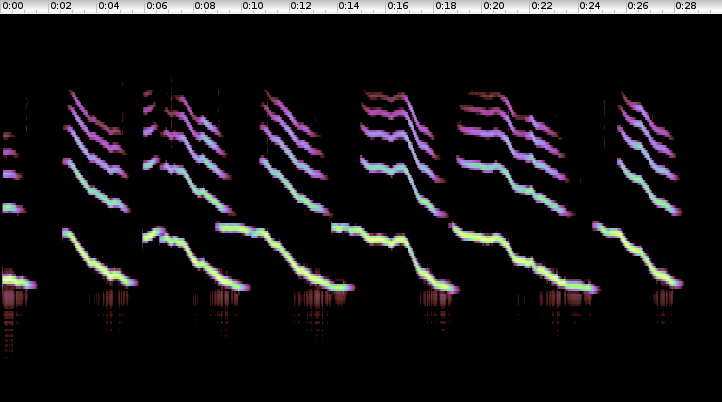
\includegraphics[width=\textwidth]{figures/blob-shaper161102.png}
\caption{Sonogram of QBO sonification with blob slice height mapped to overtone spectrum}
\label{fig:blob-shaper-161102-sono}
\end{figure}
%

\subsection{``Importing'' Timbres From a GA Process}

We have been recently experimenting with the algorithmic production of sound synthesis structures, by using genetic programming of synth graphs based on a target sound and a fitness function that correlates the spectra and loudness contours of target sound and individuals in the GP populations. While this does not yield sounds close to the target sound in reasonable time and number of iterations, it has proven to be a very useful generator of interesting timbres.

Therefore, it seems useful to try and ``import'' timbres produced in this evolutionary algorithm to SysSon. There is a simple source code generator for the found sound structures, and the work is then to select a sound, unclutter the source code from ``dead'' branches (e.g. those that essentially produce silence or components that one wants to remove from the timbre), and finally identify parameters that one wants to control (e.g. fundamental frequency). The GP comes up with interesting solutions for modulating timbre, such as adding signals and then clipping the sum, producing thus co-modulations.

\figref{fig:code-shaper-timbre2} shows the result of such an imported sound, with the sonogram for applying it in the usual QBO setup shown in \figref{fig:sono-shaper-timbre2}. A bounce of this sound can be found at \url{https://soundcloud.com/syssonproject/blob-shaper-timbre2-161107}.

\begin{figure}[b]
\begin{lstlisting}[style=scala]

// ---- oscillator ----

def mkOsc1(freq: GE): GE = SinOsc.ar(freq) * 0.75

def mkOsc2(freq: GE): GE = {
  val freq_4          = freq
  
  val amt_1           = 0.1
  val off_1           = 0.7
  val amt_2           = 1.0
  val freq_3          = 0.6 // adds irregularity
  val freq_5          = (freq_4 * 2).min(18000) // lpf
  
  val lFCub_0         = LFCub.ar(freq = freq_3, iphase = 0.660289)
  val min_7           = lFCub_0.min(0.0)
  val lFDNoise0       = LFDNoise0.ar(freq_3) + off_1
  val gbmanL          = GbmanL.ar(freq = freq_4, xi = 383.95047, yi = 383.95047)
  val min_33          = gbmanL min 0.36345935
  val blip            = Blip.ar(freq = freq_4, numHarm = 1.0)
  val plus            = blip + 0.1321
  val mix             = Mix(Seq[GE](
      lFDNoise0 * amt_1, 
      min_7 * amt_2, 
      min_33, 
      plus
  ))
  val sig0 = LeakDC.ar(mix.clip2(1)) * 0.75
  val sig  = LPF.ar(sig0, freq_5)
  sig
}

def mkOsc(freq: GE, amt: GE): GE = {
  val numOscs = 2
  val oscs = Seq(mkOsc1(freq), mkOsc2(freq))
  
  val idx  = amt.linlin(0, 1, 0, numOscs - 1)
  val idxF = idx.floor
  val idxC = idx.ceil
  val wC   = idx % 1.0
  val wF   = 1.0 - wC
  
  val osc  = Select.ar(idxF, oscs) * wF + Select.ar(idxC, oscs) * wC
  osc
}
\end{lstlisting}
\caption{Oscillator mix by fading between sine and complex timbre.}
\label{fig:code-shaper-timbre2}
\end{figure}

\begin{figure}
\centering
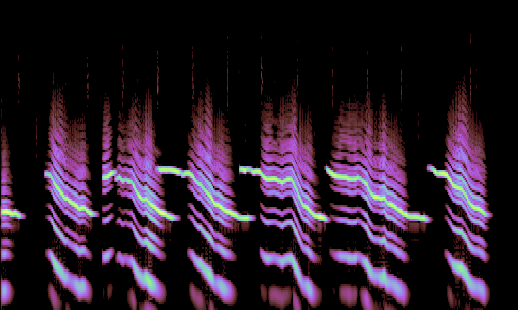
\includegraphics[width=0.75\textwidth]{figures/blob-shaper-timbre2-161106.png}
\caption{Sonogram of QBO sonification with fading between sine and complex timbre.}
\label{fig:sono-shaper-timbre2}
\end{figure}

\figref{fig:code-shaper-timbre3} shows the result of another such imported sound, with the sonogram for applying it in the usual QBO setup shown in \figref{fig:sono-shaper-timbre3}. A bounce of this sound can be found at \url{https://soundcloud.com/syssonproject/blob-shaper-timbre3-161107}.

\begin{figure}[b]
\begin{lstlisting}[style=scala]
def mkOsc1(freq: GE): GE = SinOsc.ar(freq) * 0.75

def mkOsc3(freq: GE): GE = {
  val freq1 = freq
  val amt1  = 0.125 // modulation
  val freq2 = 13.0
  val freq3 = (freq1 * 3.0).min(18000)
  
  val gbmanL_0        = GbmanL.ar(freq = freq1, xi = 383.95047, yi = 383.95047)
  val blip            = Blip.ar(freq = freq1, numHarm = 1)
  val min_3           = -0.058492452
  val difsqr          = blip difsqr min_3
  val ring2           = gbmanL_0 ring2 difsqr
  val min_4           = 0.660289 min ring2
  val min_5           = min_4 min -0.058492452
  val b               = gbmanL_0.min(0.0)
  val min_6           = b min gbmanL_0
  val a               = min_4 min min_6
  val decayTime_1_X   = QuadN.ar(freq = 0.660289, a = a, b = b, c = min_4, xi = min_5)
  val decayTime_1 = decayTime_1_X.clip2(770)
  val in_3            = LeakDC.ar(decayTime_1)
  val min_10          = min_6.min(0.0)
  val in_4            = LeakDC.ar(min_10)
  val combL           = CombL.ar(in_4, maxDelayTime = 0.0, 
    delayTime = 0.0, decayTime = 0)
  val min_11          = combL min min_6
  val min_13          = min_11 min min_6
  val min_15          = min_5 min min_13
  val min_16          = min_15.min(0.0)
  val in_6            = LeakDC.ar(difsqr)
  val allpassC        = AllpassC.ar(in_6, maxDelayTime = 0.01,
    delayTime = 0.01, decayTime = decayTime_1)
  
  val mix0 = min_16 * amt1 + allpassC
  val mix = LPF.ar(mix0, freq3)
  LeakDC.ar(mix.clip2(1)) * 0.75
}  

def mkOsc(freq: GE, amt: GE): GE = {
  val numOscs = 2
  val osc1 = mkOsc1(freq)
  val osc3 = mkOsc3(freq)
  val oscs = Seq(osc1, osc1 * 0.5 + osc3)
  val idx  = amt.linlin(0, 1, 0, numOscs - 1)
  val idxF = idx.floor
  val idxC = idx.ceil
  val wC   = idx % 1.0
  val wF   = 1.0 - wC
  val osc  = Select.ar(idxF, oscs) * wF + Select.ar(idxC, oscs) * wC
  osc
}
\end{lstlisting}
\caption{Oscillator mix -- timbre 3.}
\label{fig:code-shaper-timbre3}
\end{figure}

\begin{figure}
\centering
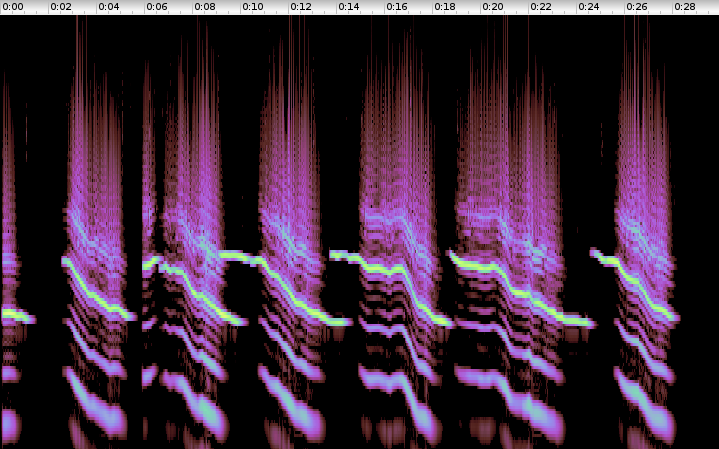
\includegraphics[width=\textwidth]{figures/blob-shaper-timbre3-161107.png}
\caption{Sonogram of QBO sonification with fading between sine and complex timbre.}
\label{fig:sono-shaper-timbre3}
\end{figure}

\figref{fig:code-shaper-timbre4} shows the result of another such imported sound, with the sonogram for applying it in the usual QBO setup shown in \figref{fig:sono-shaper-timbre4}. A bounce of this sound can be found at \url{https://soundcloud.com/syssonproject/blob-shaper-timbre4-161107}. Here we fade between three different mixes and with wider overlap, resulting in less discernible ``stages'', but perhaps also leading to more difficulties in ``categorising'' the sound.

\begin{figure}[b]
\begin{lstlisting}[style=scala]
def mkOsc4(freq: GE): GE = {
  val freq3 = freq
  val freq2 = 3615.845
  val freq1 = 10.285505 // modultion freq
  val amt1  = 0.2 // modulation depth
   
  val saw_0           = Saw.ar(freq1) * amt1
  val a_2             = BrownNoise.ar.linlin(-1, 1, 0.3, 0.85)
  val latoocarfianL   = LatoocarfianL.ar(freq = freq2, a = a_2, b = 1.5, c = 0.5, d = 0.0,
    xi = -1.8525897, yi = saw_0)
  val ratio = freq3 / (2.0 * 349.2)
  val shift            = PitchShift.ar(latoocarfianL, pitchRatio = ratio) * 1.5
  val mix = Resonz.ar(shift, freq3 * 1.1) * 1.41
  mix
}
  
def mkOsc(freq: GE, amt: GE): GE = {
  val numOscs = 3
  val osc1 = mkOsc1(freq)
  val osc2 = mkOsc2(freq)
  val osc3 = mkOsc3(freq)
  val osc4 = mkOsc4(freq)
  
  val mix1 = osc1
  val mix2 = osc1 * 0.5 + osc2 * 0.5
  val mix3 = osc4 + osc3 * 0.33
  
  val idx  = amt.linlin(0, 1, 0, numOscs - 1)
  val mix1w = mix1 * (1.4 - idx.absdif(0).clip(0, 1.4).sqrt)
  val mix2w = mix2 * (1.4 - idx.absdif(1).clip(0, 1.4).sqrt)
  val mix3w = mix3 * (1.4 - idx.absdif(2).clip(0, 1.4).sqrt)
  val osc =  mix1w + mix2w + mix3w
  osc * 0.7
}
\end{lstlisting}
\caption{Oscillator mix -- timbre 4 (functions 'mkOsc1', 'mkOsc2', 'mkOsc3' as before).}
\label{fig:code-shaper-timbre4}
\end{figure}

\begin{figure}
\centering
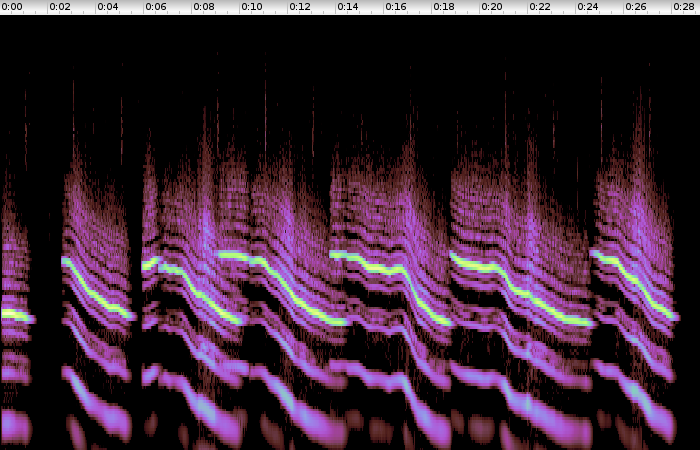
\includegraphics[width=\textwidth]{figures/blob-shaper-timbre4-161107.png}
\caption{Sonogram of QBO sonification with fading between sine and complex timbre.}
\label{fig:sono-shaper-timbre4}
\end{figure}

\subsection{Evaluation}

After refinements, the sounds chosen for the meeting on 10-Nov-2016 have been uploaded to \url{https://soundcloud.com/syssonproject/sets/wegc_161110-neu}. Descriptions:

\paragraph{QBO Blob - Timbre1 (Just Sine)}:
Anomalies based on \Verb!"5x30-climatology_2001-05-01_2016-05-01_ta"!; time slice = 0 to 179 (2001-05-16 12:00:00Z to 2016-04-16 00:00:00Z); lon = 75 deg W; lat = 2.5 deg S. Using blob analysis of altitudes 20 km to 40 km.
%
\begin{itemize}
\item time is mapped to time (2, 6, and 12 months per second)
\item altitude is mapped to pitch (20 km = 300 Hz, 40 km = 800 Hz).
\item only hot anomalies are filtered
\item frequency is determined as centroid (weighted mean) of altitude bands within blob
\item strength of centroid band is indicated by amplitude of sound generator
\end{itemize}

\paragraph{QBO Local - Max Trajectory}:
Anomalies based on \Verb!"5x30-climatology_2001-05-01_2016-05-01_ta"!; time slice = 0 to 179 (2001-05-16 12:00:00Z to 2016-04-16 00:00:00Z); lon = 75 deg W; lat = 2.5 deg S. Using one oscillator per signum with frequency corresponding to altitude between 21 km to 39 km that exhibits the strongest anomaly.
%
\begin{itemize}
\item time is mapped to time (2, 6, 12 months per second)
\item altitude is mapped to pitch (21 km = 200 Hz, 39 km = 4 kHz).
\item hot anomalies are projected onto the left channel
\item cold anomalies are projected onto the right channel (using the same frequency mapping as for hot anomalies)
\item frequency is determined as altitude band with maximum anomaly
\item strength of maximum band is indicated by amplitude of oscillator
\end{itemize}

\paragraph{QBO Cluster}:
Anomalies based on \Verb!"5x30-climatology_2001-05-01_2016-05-01_ta"!; time slice = 0 to 179 (2001-05-16 12:00:00Z to 2016-04-16 00:00:00Z); lon = 75 deg W; lat = 2.5 deg S. Using oscillator bank with one oscillator per altitude, filtering only hot anomalies.
%
\begin{itemize}
\item time is mapped to time (2, 6, 12 months per second)
\item altitude is mapped to a fixed pitch (20 km = 200 Hz, 40 km = 4 kHz; logarithmically) for each oscillator (N altitude bands = N oscillators).
\item hot anomalies of >1 degrees are filtered
\item strength of each oscillator reflects anomaly strength from threshold
(1 degree; minimum amplitude) to a given maximum of 8 degrees (maximum amplitude).
\end{itemize}

\paragraph{QBO Blob - Timbre1}:
Anomalies based on \Verb!"5x30-climatology_2001-05-01_2016-05-01_ta"!; time slice = 0 to 179 (2001-05-16 12:00:00Z to 2016-04-16 00:00:00Z); lon = 75 deg W; lat = 2.5 deg S. Using blob analysis of altitudes 20 km to 40 km.
%
\begin{itemize}
\item time is mapped to time (2, 6, 12 months per second)
\item altitude is mapped to pitch (20 km = 300 Hz, 40 km = 800 Hz).
\item only hot anomalies are filtered
\item fundamental frequency is determined as centroid (weighted mean) of altitude bands within blob
\item timbre (richness is overtones or brightness of sound) is determined by blob height (span from low to high altitudes including the centroid and exceeding temperature threshold)
\item strength of centroid band is indicated by amplitude of sound generator
\end{itemize}

\paragraph{QBO Blob - Timbre2 - 0.5 Factor}:
Anomalies based on \Verb!"5x30-climatology_2001-05-01_2016-05-01_ta"!; time slice = 0 to 179 (2001-05-16 12:00:00Z to 2016-04-16 00:00:00Z); lon = 75 deg W; lat = 2.5 deg S. Using blob analysis of altitudes 20 km to 40 km.
%
\begin{itemize}
\item time is mapped to time (6 months per second)
\item altitude is mapped to pitch (20 km = 300 Hz, 40 km = 800 Hz).
\item only hot anomalies are filtered
\item fundamental frequency is determined as centroid (weighted mean) of altitude bands within blob
\item timbre is determined by blob height (span from low to high altitudes including the centroid and exceeding temperature threshold): narrow width is audible as a "plain" sine tone, higher widths are indicates by an additional "rough" timbre in a frequency register around three octaves below the sine indicating the centroid.
\item strength of centroid band is indicated by amplitude of sound generator
\end{itemize}

\paragraph{QBO Blob - Timbre2 - 2.0 Factor}:
Anomalies based on \Verb!"5x30-climatology_2001-05-01_2016-05-01_ta"!; time slice = 0 to 179 (2001-05-16 12:00:00Z to 2016-04-16 00:00:00Z); lon = 75 deg W; lat = 2.5 deg S. Using blob analysis of altitudes 20 km to 40 km.
%
\begin{itemize}
\item time is mapped to time (6 months per second)
\item altitude is mapped to pitch (20 km = 300 Hz, 40 km = 800 Hz).
\item only hot anomalies are filtered
\item fundamental frequency is determined as centroid (weighted mean) of altitude bands within blob
\item timbre is determined by blob height (span from low to high altitudes including the centroid and exceeding temperature threshold): narrow width is audible as a "plain" sine tone, higher widths are indicates by an additional "rough" timbre in the same frequency register as the sine indicating the centroid.
\item strength of centroid band is indicated by amplitude of sound generator
\end{itemize}

\paragraph{QBO Hot - Cold Figurative}:
Anomalies based on \Verb!"5x30-climatology_2001-05-01_2016-05-01_ta"!; time slice = 0 to 179 (2001-05-16 12:00:00Z to 2016-04-16 00:00:00Z); lon = 75 deg W; lat = 2.5 deg S. Using one sound generator per signum with frequency corresponding to altitude between 21 km to 39 km that exhibits the strongest anomaly.
%
\begin{itemize}
\item time is mapped to time (6 months per second)
\item altitude is mapped to pitch.
\item hot anomalies are projected onto the left channel, mapping
the altitude carrying maximum anomaly, between 21 km and 39 km
into the frequency range 300 to 600 Hz (logarithmically), using
a slightly noisy and sonorous timbre.
\item cold anomalies are projected onto the right channel, mapping
the altitude carrying maximum anomaly, between 21 km and 39 km
into the frequency range 1 to 2 kHz (logarithmically), using
a crispy and crackling timbre.
\item strength of maximum band is indicated by amplitude of oscillator
\end{itemize}

\paragraph{Findings:} The amplitude mapping to indicate the strength of the anomalies is rather weak. It might be a more important features, and thus the next step could be to reflect the magnitude of the anomalies more prominently, e.g. in the timbre as well. The separate timbres in the ``hot--cold'' patch are easy to distinguish when played simultaneously. It might still be useful to see if we can use the same frequency register and find timbres or other features to still tell them clearly apart. Cluster: There seem to be beatings in the sound that could stem not from the actual data but a phase-related amplitude modulation. A possible work-around might be to slightly randomise the frequencies. Andrea pointed out that some ``anomalies of anomalies'' are happening right now in 2016, the should be reflected in data starting from this spring/summer, we will see when we get updated data (current stop is April 2016).

% \printbibliography

\end{document}